\begin{frame}[t]
	\frametitle{Optimization: Dependices}

	For optimization we rely on
	\begin{itemize}
		\item 
\includegraphics[height=1cm]{images/ifopt.png}
		\item 
\includegraphics[height=2cm]{images/Ipopt.png}
	\end{itemize}
\end{frame}


\begin{frame}[fragile]
	\frametitle{Optimization: Interface}
	\begin{columns}
		\begin{column}{0.4\textwidth}
			\begin{lstlisting}[language=python]

waypoints = np.random.rand(4, 2)

c1 = broken_lines_path(waypoints)
c2 = minimum_acceleration_path(waypoints)
c3 = minimum_jerk_path(waypoints)
c4 = minimum_snap_path(waypoints)
c5 = minimum_crackle_path(waypoints)

plot2d_compare([c1, c2, c3, c4, c5], [
            'green', 'blue', 'magenta', 'red', 'black'],
            ['min vel', 'min acceleration', 'min jerk',
            'min snap', 'min crackle'])

    \end{lstlisting}
			\begin{itemize}
				\item These overshoots make these motions unreliable and collision-prone
			\end{itemize}
		\end{column}
		\begin{column}{0.6\textwidth}
			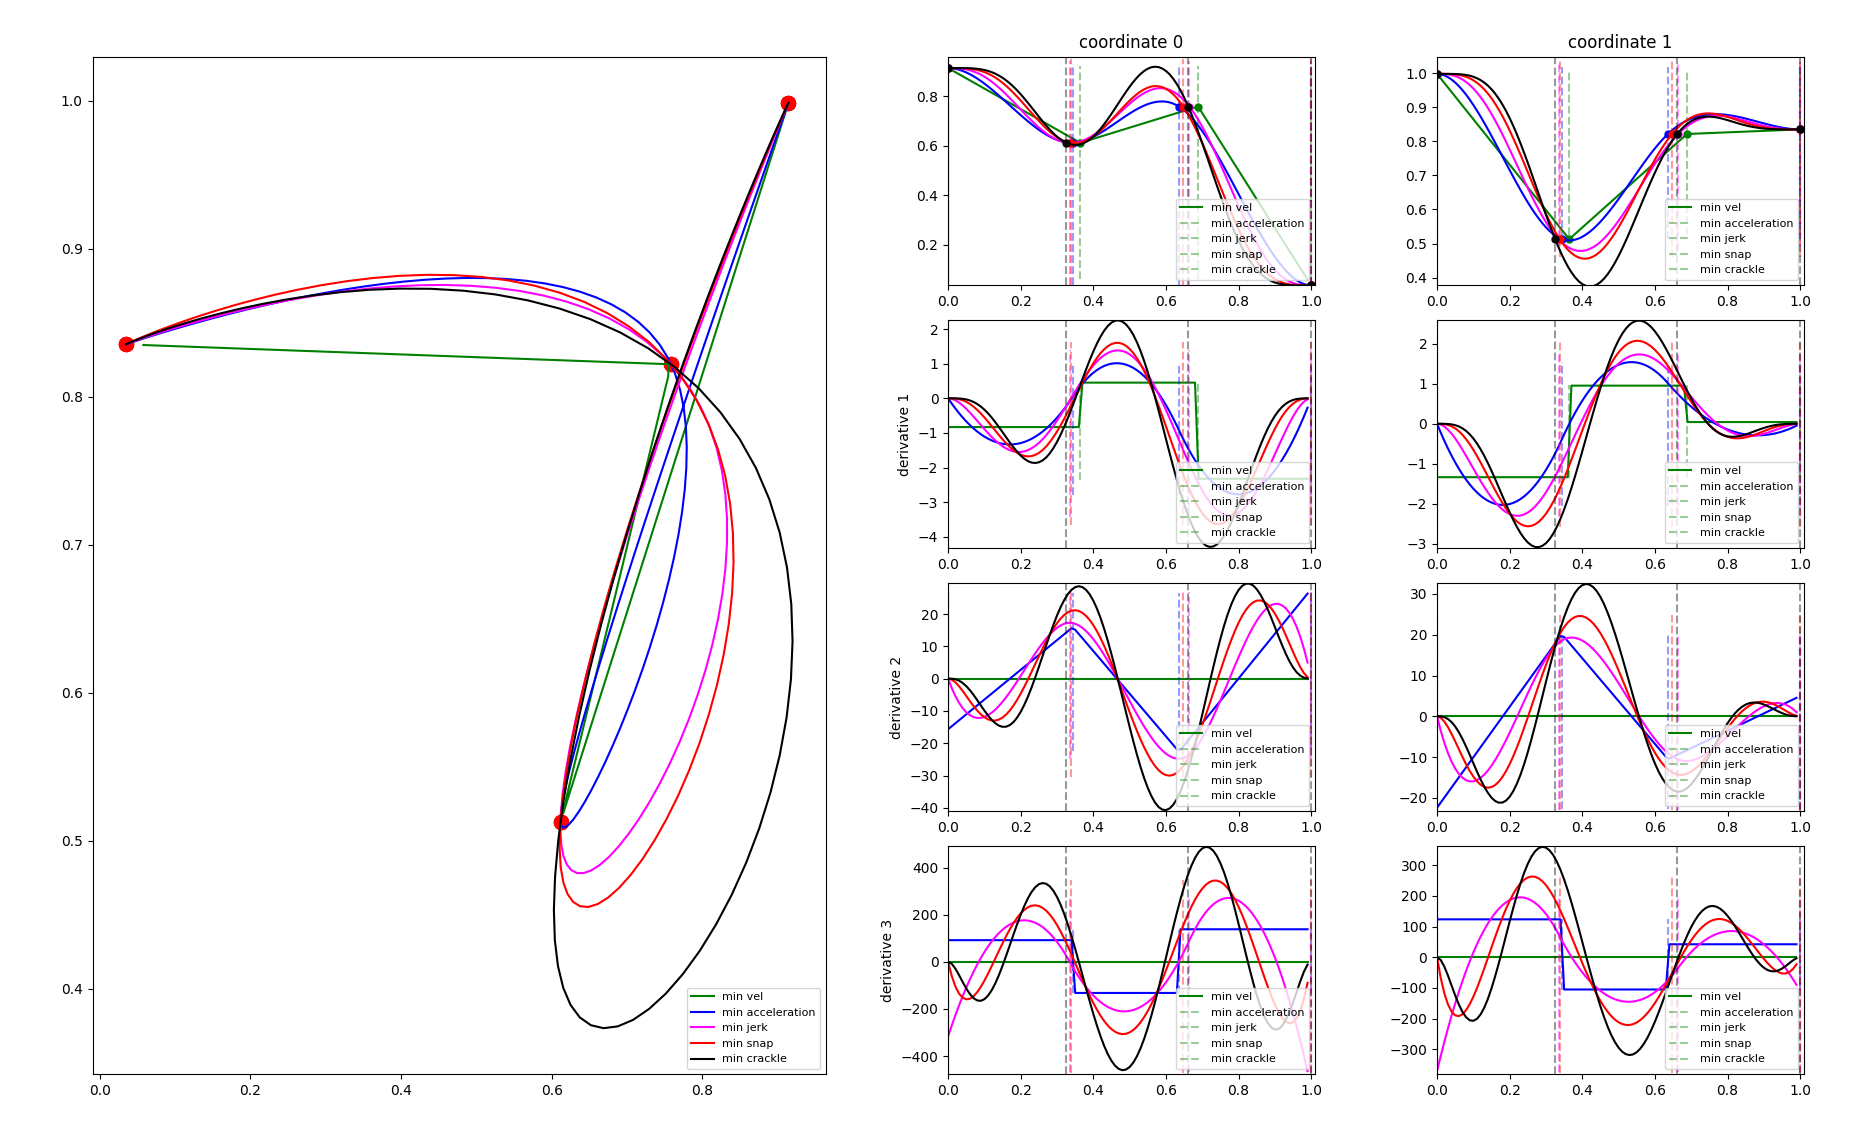
\includegraphics[width=\textwidth]{./images/comparison.png}
		\end{column}
	\end{columns}

\end{frame}
\begin{frame}[fragile]
	\frametitle{Optimization: Interface}
	\begin{columns}
		\begin{column}{0.4\textwidth}
			\begin{itemize}
				\item By balancing the jerk with the velocity we can reduce these overshoots
				      \begin{equation*}
					      \min \int_0^T \alpha \diff{\qv}{t}  + (1-\alpha) \diffk{\qv}{t}{3} \d t
				      \end{equation*}
			\end{itemize}
			\begin{lstlisting}[language=python]

waypoints = np.random.rand(4, 2)

c1 = gsplines.optimization.broken_lines_path(waypoints)
c3 = gsplines.optimization.minimum_jerk_path(waypoints)
c4 = gsplines.optimization.rojas_path(waypoints, 0.8)
c5 = gsplines.optimization.rojas_path(waypoints, 1.5)
c6 = gsplines.optimization.rojas_path(waypoints, 2)

gsplines.plot.plot2d_compare([c1, c3, c4, c5, c6], [
            'green', 'blue', 'magenta', 'red',
            'gray'],
            ['min vel', 'min jerk', 'balance k=0.8',
            'balance k=1.5', 'balance k=2'])
\end{lstlisting}
		\end{column}
		\begin{column}{0.6\textwidth}
			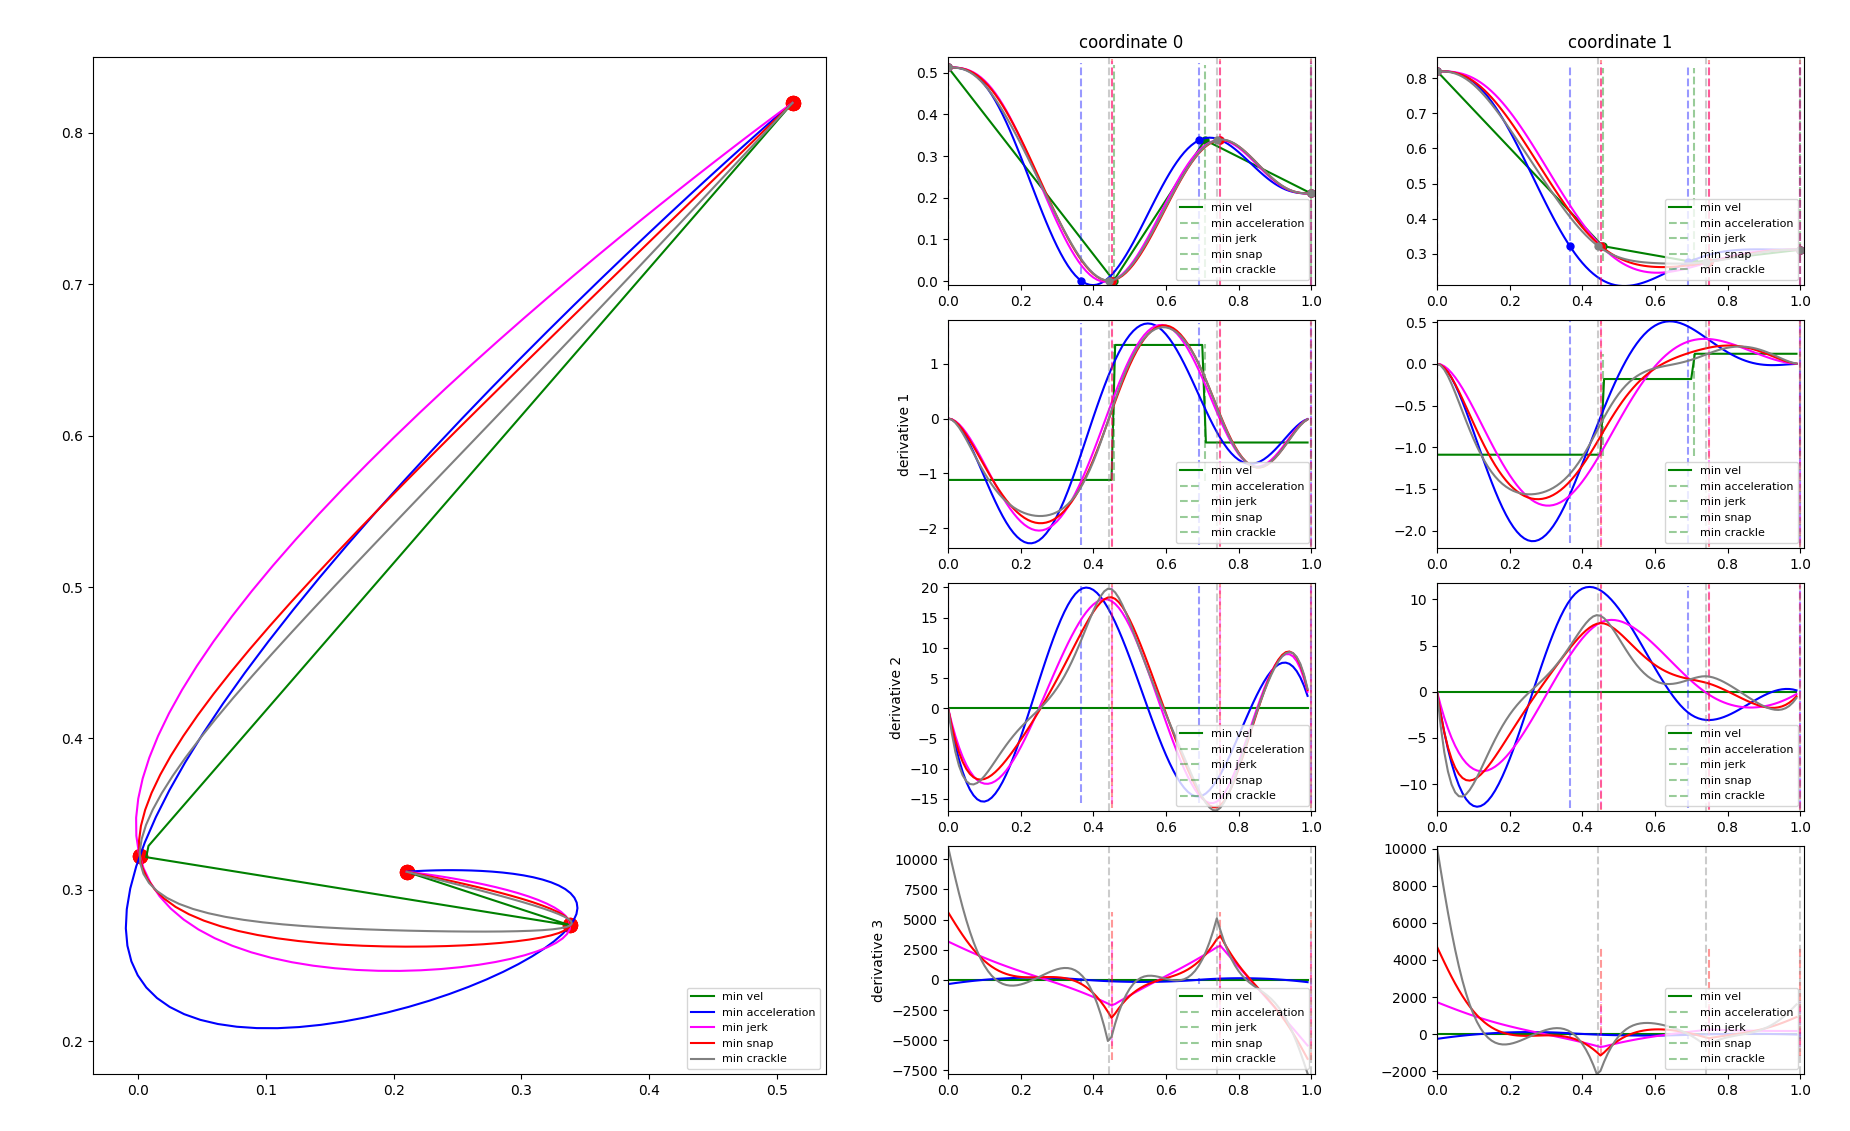
\includegraphics[width=\textwidth]{./images/comparison_2.png}
		\end{column}
	\end{columns}

\end{frame}


\begin{frame}
	\frametitle{A better type of motions}
	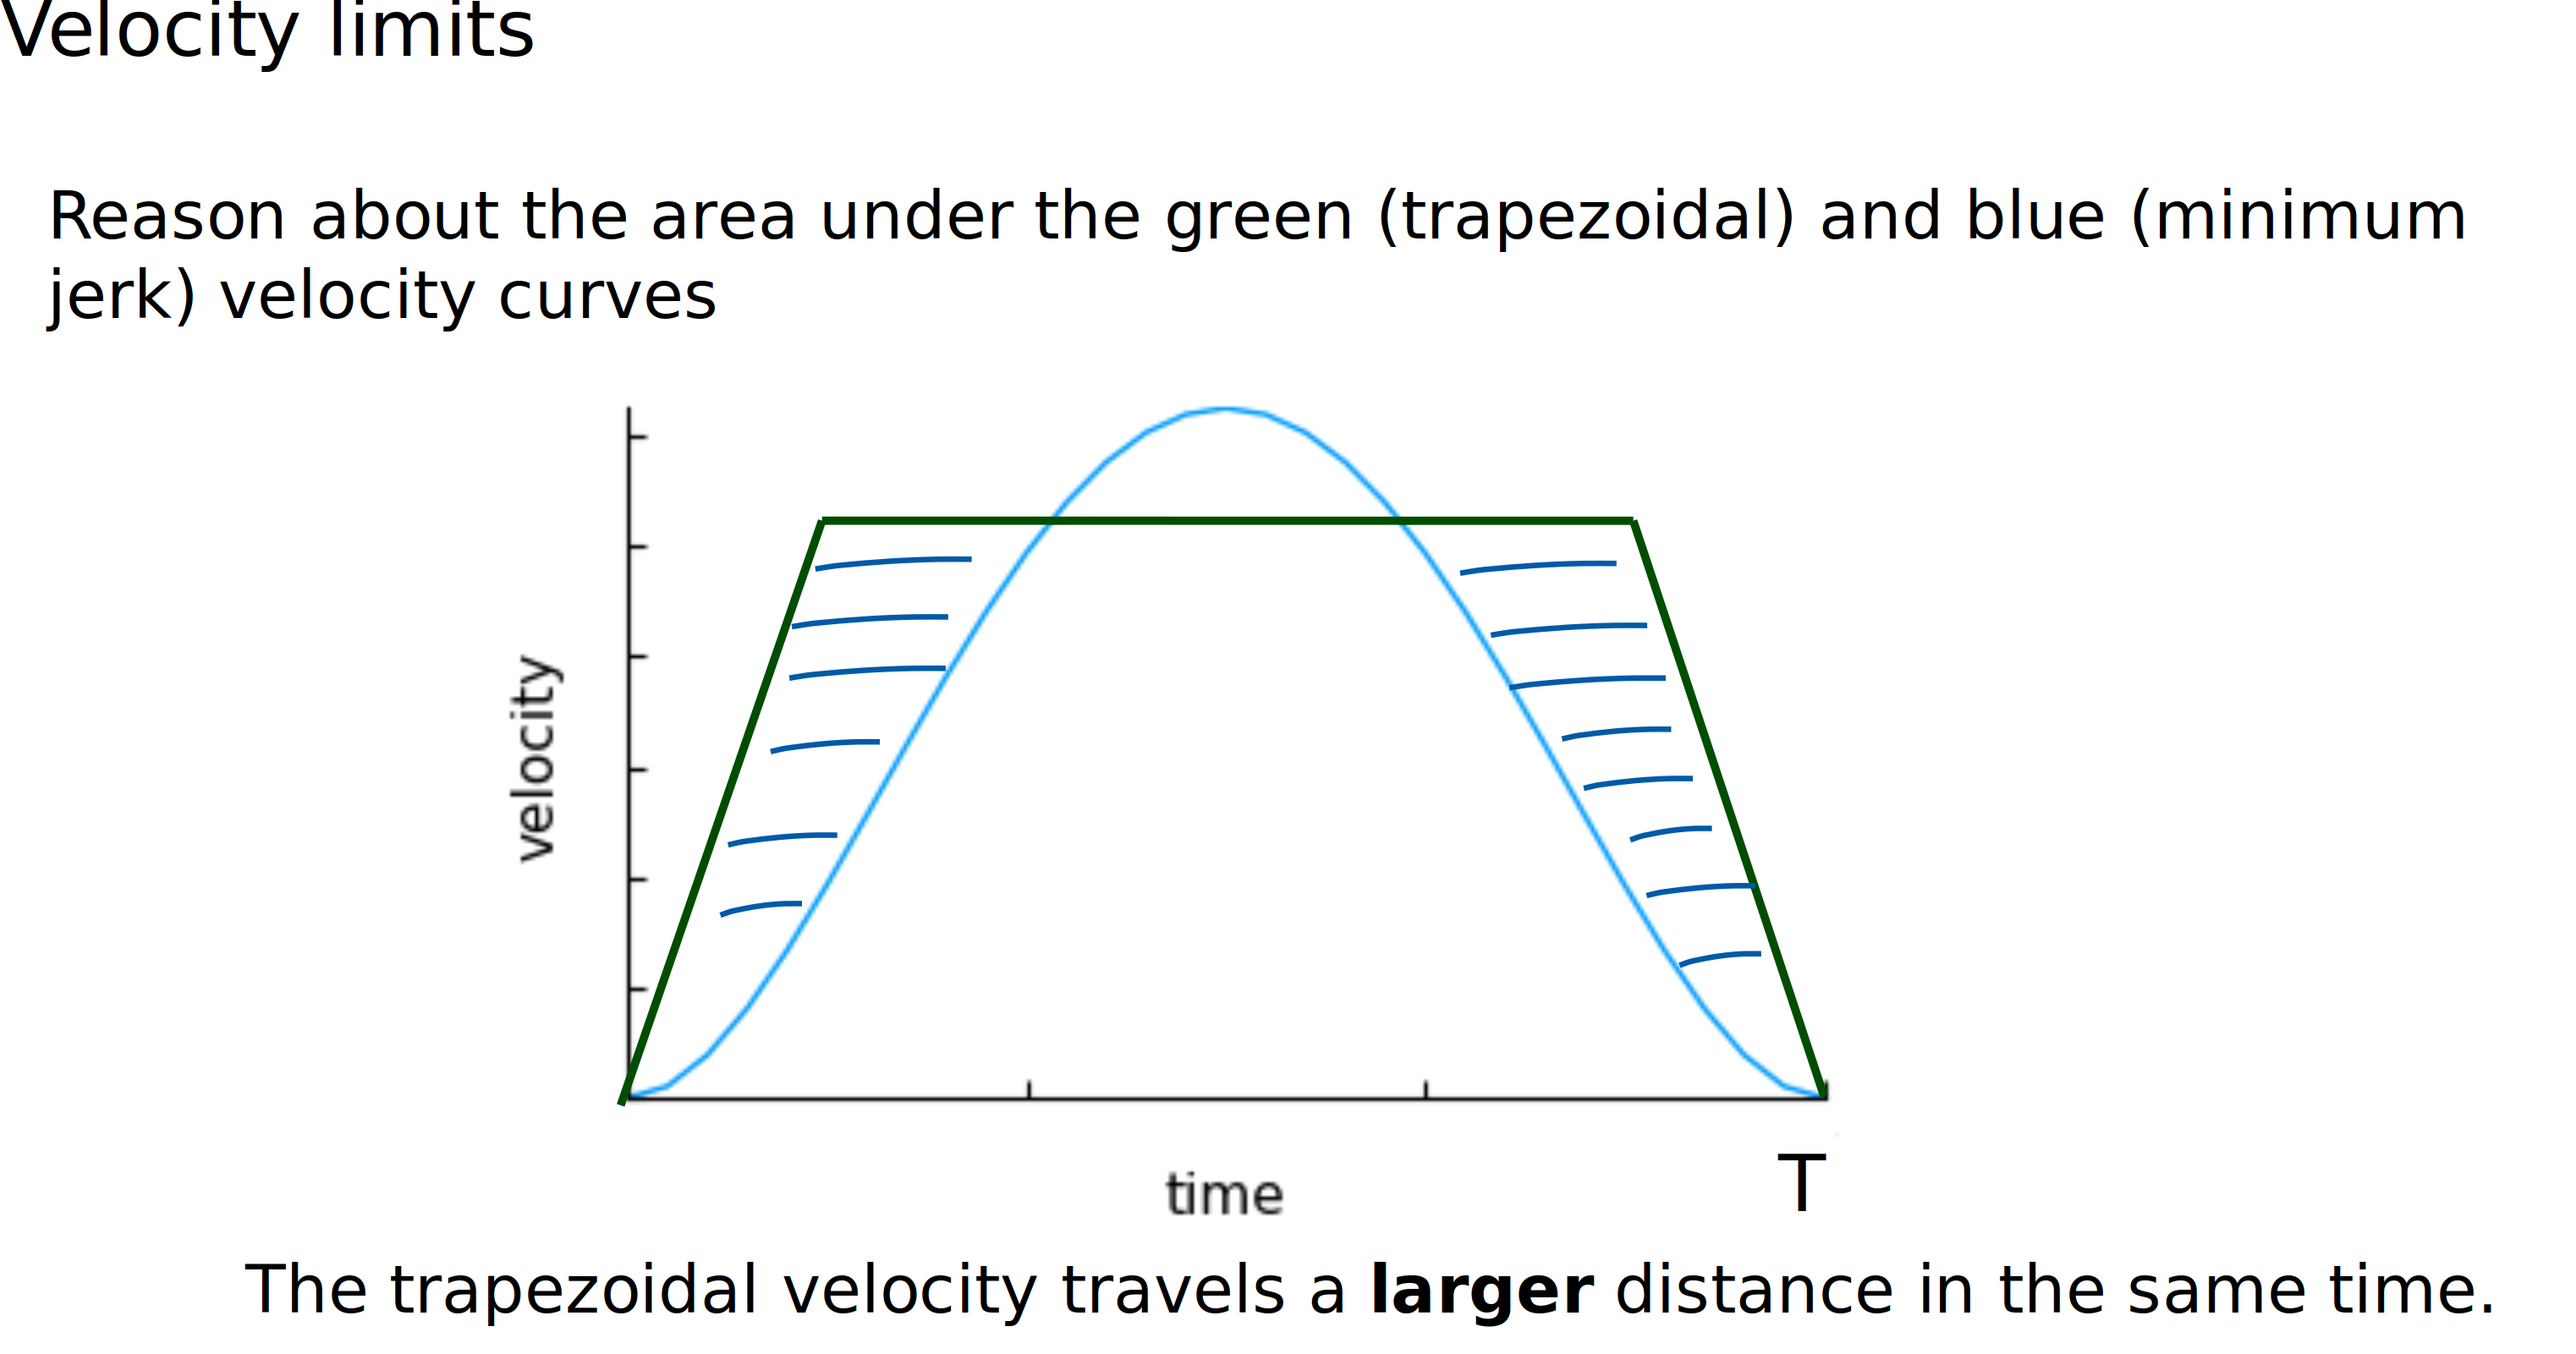
\includegraphics[width=\textwidth]{./images/temporal_slide_trapezoidal_and_corners.png}
\end{frame}

\begin{frame}
	\frametitle{Comparison with Ruckig and Pilz}
\end{frame}

\begin{frame}[fragile]
	\frametitle{OpStop: Interface}
	\begin{columns}
		\begin{column}{0.4\textwidth}
			\begin{lstlisting}[language=python]
import gsplines
import gsplines.plot as gplot
import numpy as np
import opstop
from gsplines.optimization import minimum_jerk_path


model_file = 'path_to_urdf_robot_description'

dim = 7   # number of joints of the robot
# Generate a random numpy array of wayponts
# (each row is a waypoint in R^n)
number_of_waypoints = 5
waypoints = np.random.rand(number_of_waypoints, dim)
# The a minimum jerk trajectory with execution time of 5s
trj = minimum_jerk_path(waypoints).linear_scaling_new_execution_time(5.0)
# Select the time to stop as the 60% of the time.
stop_ti = trj.get_domain()[1]*0.6
# Get a parametrization that minimizes the time and  does not
# allow an increment in the acceleration larger than 50%
optimal_parametrization = opstop.minimum_time_bounded_acceleration(
    trj, stop_ti, 1.5, str(model_file), 8)
# Obtain the stopping trajectory
stop_trj = trj.compose(optimal_parametrization)
# Plot the nominal and the stopping trajectory
gplot.plot_compare([stop_trj, trj], ['red', 'blue'], [
                       'Emergency Stop Trajectory',
                                          'Original Trajectory'], _show=True, _up_to_deriv=2)
    \end{lstlisting}
		\end{column}
		\begin{column}{0.6\textwidth}
			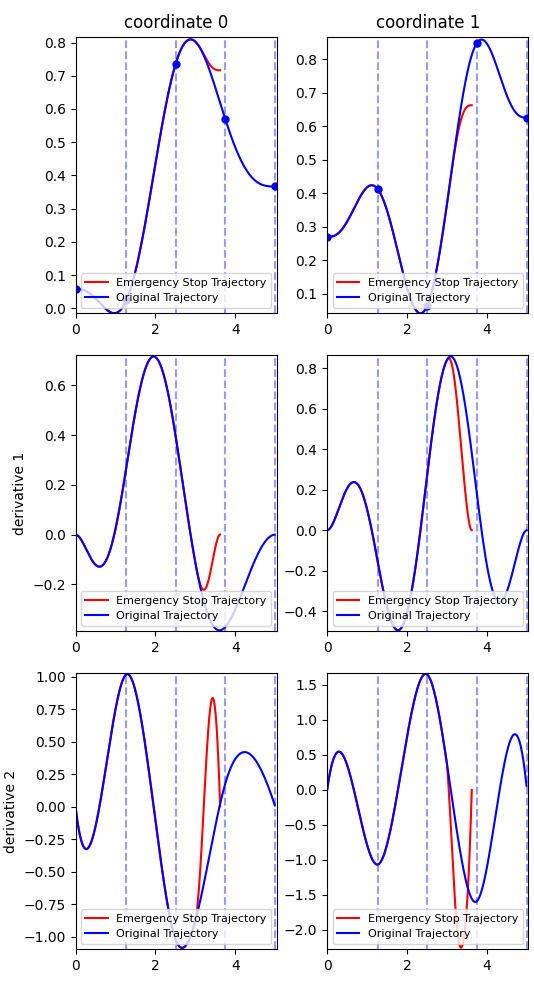
\includegraphics[width=3cm]{./images/temporal_opstopimage.png}
		\end{column}
	\end{columns}
\end{frame}
\begin{frame}
	\frametitle{OpStp}
\end{frame}
